\newpage\section{Theoretical foundations}

This section represents the theoretical fundamentals of this elaboration by defining the term \enquote{data analytic}, the concept of the \enquote{information value chain}, the \ac{dsr} methodology, the \textit{requirement engineering} approach and the experimental research process in general.

%\subsection{Definition of terms}

\subsection{Data Analytics}

The term \enquote{data analytics} originated in the early 2000s and describes an interdisciplinary field that combines areas such as statistics, machine learning, pattern recognition, system theory, operations research and artificial intelligence \parencite{Runkler.2020}. It can be generally defined \enquote{[...] as the application of computer systems to the analysis of large data sets for the support of decisions.} \parencite{Runkler.2020}. This definition showcases the broadness of the topic, as most computer systems process some amount of data and thus theoretically allow for some kind of decision making. Due to this broad definition, data analytics can cover slightly different subject areas depending on the context it is discussed in. In this elaboration, data analytics refers to the processing of large amounts of data, also referred  to as \enquote{big data}, through mathematical procedures or machine learning methods with the goal of creating new knowledge. Subsequently, processes that merely prepare or show data are not considered data analytics, but only processes that process data in such a way that new knowledge can be derived from it. This distinction is made to differentiate data analytics from traditional data processing areas like business intelligence. The goal of data analytics, as is discussed in this thesis, is to retrieve some kind of previously unknown knowledge from a set of data. This process can be generally described using the \enquote{information value chain} model. In their research, Abbasi et al. analyze this model in the context of big data in an effort to create an inclusive research agenda for big data in information system research \parencite{Abbasi.2016}.

\subsection{Information Value Chain}
\label{subsec:informationValueChainSubSection}

The information value chain (figure \ref{information_value_chain}) is a set of phases that define the transformation of raw data to information and eventually into knowledge. \enquote{Data} describes raw facts without any structuring. Once organized, the processed data represents \enquote{information}. This \enquote{information} is then used to find patterns and draw conclusions. At this time, the information becomes knowledge \parencite{Fayyad.1996}, \cite{Fayyad.1996b}. This knowledge is then used to make \enquote{decisions} and take corresponding \enquote{actions} \parencite{Sharma.2014}. Each phase of the information value chain also includes a different set of technologies and methodologies. For example, the \enquote{data} phase contains technologies and actions regarding the basic storage of data like database systems or data warehouses \parencite{Abbasi.2016}. The conventional version of this information value chain represents an approach that generally explains the processing of data. The main steps of this information value chain are also applicable for big data \parencite{Abbasi.2016}. This general structure of processing data is also supported by literature from the data analytics field \parencite{Runkler.2020}. In addition, the information value chain contains the further phases \enquote{decisions} and \enquote{actions}, which deal with the influence of the processed data. These phases reflect the impact of data analytics, since data analytics is primarily a technology for the decision-making process \parencite{Runkler.2020}. For this reason, the information value chain is a suitable model to structure different phases in the processing of data in the context of data analytics. %For this reason, the literature examined in this paper is structured according to the phases of the information-value chain.



\begin{figure}[]
    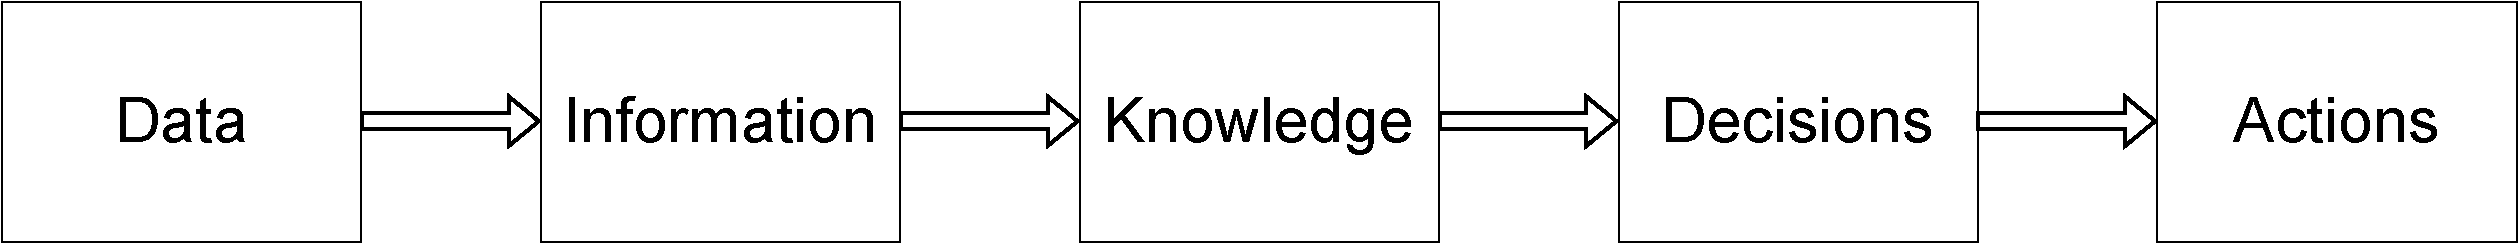
\includegraphics[width=0.99\textwidth, keepaspectratio]{content/02_theretical_foundations/informationValueChain.pdf}
    \caption{Information Value Chain}    
    \label{information_value_chain}
\end{figure}

%\subsection{Boundaries and Conflicts in Organizations}

%This literature review uses the terms boundary and conflict interchangeably. In order to include as much literature as possible, the criteria for boundaries are kept very general. Prior to conducting the literature review, there was no formal definition of boundaries in the context of data analytics used for the selection of literature. Generally, boundaries are described as \enquote{[...] a real or imagined line that marks the limits or edges of something and separates it from other things or places [...]} \parencite{Hornby.2015}. Based on this general description, the term boundary is defined in the context of this elaboration as any circumstance that leads to a reduction in the effectiveness or efficiency of an organization. %Based on this description, the term \enquote{boundary} is defined in the context of this elaboration as any situation that leads to a reduction in the productivity or effectiveness of a company.
%Simultaneously, the term conflict also describes this circumstance. 
%Boundaries and conflicts are therefore used to describe any circumstance that hinders an organization from being perfectly productive. An example of such boundaries or conflicts would be communication issues between different departments, which lead to a reduction of productivity.

\subsection{Design Science Research Methodology}

In fundamental terms, design science is a research approach that aims to develop and validate science-based design knowledge and guide research to problem solving (\cite{Hevner.2004}, \cite{Dresch.2015}). The goal of \ac{dsr} is to gain prescriptive knowledge about the composition of various artifacts, including software, methods, models, and concepts. This particular design knowledge facilitates a systematic and scientific approach to the design of future projects. The design process and its practical implementation generate design-oriented knowledge, enriching the existing knowledge in \ac{dsr} (\cite{Hevner.2004}). Thus the result of design-science, especially in \ac{is}, is the creation of an effective \ac{it} artefact which deals with a certain problem (\cite{Hevner.2004}), making the \ac{dsr} a suitable approach for this thesis. Nevertheless, the exact activities of the design science model may differ from author to author to some extent (\cite{Fulcher.1996}). This thesis aligns itself with the phases and steps outlined by Peffers et al. in their 2006 article \enquote{The design science research process: A model for producing and presenting information systems research}. In their article Peffers et al. analyze literature that implements design science in order to create a generally accepted process for research in \ac{is} (\cite{Peffers.2006}). As a result of their work, they describe the design science research approach using the following six steps: (\cite{Peffers.2006}) 

\begin{enumerate}
    \item \textbf{\textit{Identification of the Problem}}: In this phase, the problem fundamentally solved by the resulting artifact is described. At the same time the value of resulting solution is justified. %The problem identification in this thesis is realized through a literature search which focusses on boundaires and conflicts that limit the utilization of data analyitics.
    \item \textbf{\textit{Definition of Objectives for a solution}}: This phase focuses on the specific goal of the solution and how its solving can be measured. The objectives for the solution can usually be divided into qualitative and quantitative characteristics. 
    \item \textbf{\textit{Design and Dev of artefacts}}: This step covers the specific functional design and scope of the artifact and how it is to be achieved. The phase covers both the conceptual design and the specific practical implementation of the solution.
    \item \textbf{\textit{Demonstration of the Artifact}}: The focus of this phase is to demonstrate that the artifact implemented in the previous step can actually solve the initial problem. For this purpose, various methods such as experiments, case studies or other test setups can be used.
    \item \textbf{\textit{Evaluation of the solution}}: This step evaluates the artifact and measures how well it contributes to a solution to the problem, therefore this phase tests whether the developed artefact is a valid solution to the research problem. If the artifact does not meet the corresponding requirements, the process is iterated back to step number three. If the artifact meets all requirements and contributes significantly to the solution of the problem, the last step is conducted. 
    \item \textbf{\textit{Communication}}: The last step ensures that the developed artefact and its value is communicated to the scientific community. The goal of this phase can be achieved through a number of different ways. The choice for the right way of communicating the results thereby relies on the specific topic and problem at hand.
\end{enumerate}



%The first step, \textit{Identification of the Problem}, \enquote{Define the specific research problem and justify the value of a solution.} (\cite{Peffers.2006}). The 

%Peffers et al. define the phases of the \ac{dsr} methodological in their 2006 article in order  

%\cite{Fulcher.1996}


%Herbert.1996


%Originally conceived in the book \enquote{The Sciences of the Artificial} by Herbert Simon, the research approach of design science research centers primarily on the development of artifacts to solve  theoretical research problems (\cite{Dresch.2004}). 


%"The result of design-science research in IS is, by definition, a purposeful IT artifact created to address an important organizational problem. It must be described effectively, enabling its simple mentation and application in an appropriate domain." \cite{Henver.2004}



\subsection{Functional and non functional Requirements}

As a means to create any artefact, the determination of requirements are important(\cite{Seacord.2003}). Requirements can be classified according to ISO/IEC 25000, respectively the quality model from ISO/IEC 25010, as quality criteria for software and systems.(\cite{ISOIEC25010.2011}). The \ac{ieee} defines requirements as:

\begin{quote}
    \textbf{\textit{\enquote{(1) A condition or capability needed by a user to solve a problem or achieve an objective. (2) A condition or capability that must be met or possessed by a system or system component to satisfy a contract, standard, specification, or other formally imposed documents. (3) A documented representation of a condition or capability as in (1) or (2). See also: design requirement; functional requirement; implementation requirement; interface requirement; performance requirement; physical equirement.}}} \cite{IEEE.1990}
\end{quote}  
   
According to these definitions, requirements can be generally defined as properties that need to be met in order to achieve an objective. For this reason, the requirements for the artefact are derived from properties and characteristics of past studies in the field of data analytics. In addition, general requirements for experimental research are also taken into account. These requirements are further divided into functional and non-functional requirements. A functional requirement describes a function that a system or system component must be able to perform (\cite{IEEE.1990}). An example of a functional requirement would be the calculation of a pricetag in euros and in dollars. Non-functional characteristics describe on the other hand the behavior of a system (\cite{Seacord.2003}) and go thereby beyond the functional characteristics. Thus functional requirements describe what a system must be able to do and non-functional requirements describe how this should be done. Non-functional requirements also often describe the quality of the individual functions and can influence several other requirements (\cite{Balzert.2011}). An example of non-functional properties would be that the conversion from euros to dollars must be performed in \enquote{a few seconds}.

\subsection{Requirement Engineering}

In order to define an objective for a possible solution to the research question requirements for the created artefact must be engineered. In order to accomplishe that the \textit{requirement engineering} approach for analysis and evaluation of requirements is utilized (\cite{SWEBOK.2004}, \cite{Sommerville.2011}). This approach has been shown to clearly contribute to software project successes in the past (\cite{Hofmann.2001}) and is therefore a suitable approach to define the objectives for a solution. The exact individual phases and steps of the \textit{requirement engineering} approach can vary from source to source and use case to use case. In general, however, all steps fall into one of three main categories, the \textit{Requirements Elicitation}, \textit{Requirements Specification} and \textit{Requirements Validation} (\cite{SWEBOK.2004}, \cite{Sommerville.2011}, \cite{Fernandes.2009}). In the first step, possible requirements and use cases are collected via a variety of sources like analyses, surveys, literature or interviews (\cite{Sommerville.2011}). This thesis utilizes a literature review in order to discover requirements. In the next step, the requirements are then specified and categorized. An important distinction being the difference between functional and non-functional requirements. In the \textit{Requirements Validation} step, the elicited requirements are then tested for their validity. This phase emphasis the reviewing of the requirements in order to find out whether these requirements are actually representive of the desired artefact (\cite{Sommerville.2011}). This is accomplished througt Validity, Consistency, Completeness, Realism, and Verifiability checks in conjunction with protoyping and testing the requirements (\cite{Sommerville.2011}).


\subsection{Experiments and their research methodology}


In the context of quantitative empirical research, the starting point for experiments is a preliminary theoretical work that results in the formulation of hypotheses. These hypotheses are often found in the form that certain conditions or sets of conditions are put forward as influencing factors for a phenomenon and causal assumptions are made (\cite{Gniewosz.2011}). Experimental research and field research are often based on these causal assumptions. However, the procedure for testing these assumptions is different. In field research, phenomena (dependent variable) are supposed to be predicted by measuring influencing factors (independent variable). Independent variables or influencing factors could therefore be for example \enquote{good teaching} whereas the resulting phenomena or dependent variable would be \enquote{good grades} for the students. This posterior approach raises problems in deriving causal conclusions in many correlational studies, because effects of third variables can never be completely excluded. To address this problem, in experimental designs, the expression of the independent variable is not measured but generated by experimental manipulations. This means that the expression of the independent variable is triggered by a specific experimental design. Another key feature of experiments is the elimination of confounding variables. Confounding variables are influencing variables that can also affect the dependent variable and thus affect the relationship between the independent and dependent variable. This influence must be neutralized or controlled for the planned experiment in order to identify the effects of the independent variable (\cite{Gniewosz.2011}). There are two types of confounding variables, those that depend on the individual participants of the experiment and those that arise from the experimental design itself (\cite{Gniewosz.2011}). In order to neutralized these confounding variables a number of different approaches exist, which are listed in table \ref{tab:confounding_variables}.

\begin{table}[htbp]
    \centering
    \begin{tabular}{|L{0.49\textwidth}|L{0.49\textwidth}|}
    \cline{1-2}
    Confounding variable                                          & Description \\ \cline{1-2}
    Parallelization of confounding variables of the test subjects & The confounding variables of all test subjects are measured beforehand. the participants are then divided among the experimental conditions in such a way that the mean values of the confounding variable are approximately equal in all experimental conditions.         \\ \cline{1-2}
    Randomization of confounding variables of the subjects        & If it is not known which confounding variables might be relevant, the test subjects can be randomly assigned to experimental conditions, which from a probabilistic point of view, results in an equal distribution over the experimental conditions.     \\ \cline{1-2}
    Removing confounding variables of the experimental situation      & If it is known which experimental conditions triggers the confounding variables, these conditions should be eliminated in the experimental situation            \\ \cline{1-2}
    Keeping constant confounding variables of the experimental situation  & All confounding variables for all test subjects should have the same form         \\ \cline{1-2}
    Random variation of confounding variables of the experimental situation & If the confounding variables cannot be removed or kept constant they can be randomly assigned over the whole experimental process. The confounding variable would vary randomly between the experimental conditions and thus not be able to mask the effect of the manipulated independent variable.     \\ \cline{1-2}
    Control group                    &  Another option to rule out confounding variables is the usage of a control groups           \\ \cline{1-2}
    Control of expectation effects                   &  Not telling participants and personnel performing the experiment the final goal of the experiment can counteract expectations, which could otherwise influence the outcome as confounding variables           \\ \cline{1-2}
    \end{tabular}
    \caption[Counter measures for confounding variables]{Counter measures for confounding variables in experimental research (\cite{Gniewosz.2011})}
    \label{tab:confounding_variables}
    \end{table}

    If these confounding variables are fully removed an experiment can be conducted where the test subjects assignment to the experimental conditions is completely determined. If these confounding variables are not fully removed the effects of other influences cannot be completely ruled out. Experiments under these conditions are refered to as quasi-experiments.  
    Furthermore, there are other characteristics by which experiments are categorized. For instance Single Factorial and Multifactorial Designs describe experiments that test a single or multiple dependent variables respectively. If the independent variable is subject ot the experiment on the other hand, the experiment categories as an univariate or multivariate a design. On top of that the distinction between \enquote{between subject} and \enquote{within subject} designs are made. \enquote{Within subject} designs describe experiments where the test subjects are tested multiple times with different experimental setups, whereas \enquote{between subject} experiments test different subjects with different experimental setups (\cite{Gniewosz.2011}). 



%The scientific research process consists in large parts of the formulation of hypothesis and the testing of these hypotheses. The aim of tests being to make statements about a particular object (e.g. a person or a group of persons). These tests are usually conducted using sub-areas (also called characteristics) instead of testing the whole area (\cite{Gniewosz.2011}). One possible way of conducting tests are experiments.


